\documentclass[11pt,a4paper,final]{article} 
\usepackage[english, russian]{babel}
\usepackage[final]{pdfpages}
\usepackage{textcomp,enumitem}
\usepackage{amsmath,amsthm,amssymb}
\usepackage{fancyhdr}
\usepackage{upgreek}
\usepackage{tipa}
\usepackage{tikz}
\usepackage{graphics}
\usepackage{pgfplots}
\usepackage{indentfirst}
\usepackage[unicode, pdftex, colorlinks, urlcolor=blue]{hyperref}
\usepackage[T2A]{fontenc}
\usepackage[utf8]{inputenc} 
\usepackage[left=2cm,right=2cm,top=2cm,bottom=2cm,bindingo ffset=0cm, 
%showframe
]{geometry}
\usepackage{amsmath,amssymb,cmap,pgfplots,pgfplotstable}

\usetikzlibrary{arrows,calc,intersections}
\addto\captionsrussian{\def\refname{}}
\pgfplotsset{compat=newest}
\pgfplotsset{compat=1.9}
\linespread{1.5}
\pagestyle{plain}
\usepackage{listings}
\usepackage{listingsutf8}

\lstset{
	basicstyle=\ttfamily\small,
	keywordstyle=\color{blue},
	commentstyle=\color{green},
	stringstyle=\color{red},
	showstringspaces=false,
	breaklines=true,
	frame=single,
	inputencoding=utf8,
	literate={да}{{\cyrd\cyra}}2 {нет}{{\cyrn\cyre\cyrt}}3
}




\begin{document}
	\thispagestyle{empty}
	\begin{center}
		{\normalsize МИНОБРНАУКИ РОССИИ}
		{\normalsize ФЕДЕРАЛЬНОЕ ГОСУДАРСТВЕННОЕ БЮДЖЕТНОЕ ОБРАЗОВАТЕЛЬНОЕ УЧРЕЖДЕНИЕ}
		
		\vspace{7pt}
		
		{\normalsize ВЫСШЕГО ПРОФЕССИОНАЛЬНОГО ОБРАЗОВАНИЯ}
		
		\vspace{3pt}
		
		{\normalsize \bf <<САНКТ-ПЕТЕРБУРГСКИЙ ПОЛИТЕХНИЧЕСКИЙ УНИВЕРСИТЕТ ПЕТРА ВЕЛИКОГО>>}
		
		\vspace{1pt}
		
		{\normalsize Институт компьютерных наук и кибербезопасности}
		
		\vspace{7pt}
		
		{\normalsize Высшая школа технологий искусственного интеллекта}
		
		\vspace{7pt}
		
		{\normalsize Направление 02.03.01 Математика и компьютерные науки}
		
		\vspace{75pt}
		
		{\normalsize ОТЧЕТ О ВЫРОЛНЕНИИИ НАУЧНО-ИССЛЕДОВАТЕЛЬСКОЙ РАБОТЫ}
		
		\vspace{15pt}
		{\Large \bf Технологии параллельного программирования в
			операционных системах Linux \par}
		\vspace{55pt}
		{\normalsize }
		
		\hfill \break
		\hfill \break
	\end{center}
	
	\small{ 
		\begin{tabular}{lrrl}
			\hspace{-1cm}
			\\Студент, группа 5130201/30102 & \hspace{3cm} & \underline{\hspace{3cm}} &Санько В.В. \\\\
			\vspace{17pt}
			\hspace{-1cm}
			\\ Преподаватель: & \hspace{3cm} & \underline{\hspace{3cm}} & Чуватов М.В. \\
			\\\\
			&&\hspace{5cm}
		\end{tabular}
		\begin{flushright}
			<<\underline{\hspace{1cm}}>>\underline{\hspace{2.5cm}} 2025г.
		\end{flushright}
	}
	
	\hfill \break
	\hfill \break
	\begin{center} \small{Санкт-Петербург, 2025} \end{center}
	\thispagestyle{empty}
	

\newpage
\section*{РЕФЕРАТ}
\addcontentsline{toc}{section}{РЕФЕРАТ}

Отчет 62 с., 9 рис., 1 табл., 7 источников, 1 прил.

\textbf{ПАРАЛЛЕЛЬНОЕ ПРОГРАММИРОВАНИЕ, LINUX СИСТЕМЫ, ТЕХНОЛОГИЯ OPENMP, ТЕХНОЛОГИЯ OPENMPI, АЛГОРИТМЫ ТЕОРИИ ГРАФОВ}

Объектом исследования являются технологии параллельного программирования в операционных системах на базе ядра Linux.

Цель работы — проектирование сети компьютеров и разработка терминального приложения, реализующего алгоритмы теории графов с применением методов параллельного программирования.

В процессе работы установлены виртуальная среда VirtualBox и операционная система AlmaLinux. Проведена настройка сети, изучены технологии OpenMP и OpenMPI. Разработано приложение на языке C++, реализующее параллельные версии алгоритмов теории графов.

В результате исследования создано приложение, корректно запускающееся на сети компьютеров. Реализованы алгоритмы для подсчёта количества остовных деревств с помощью матричной теоремы Кирхгофа, поиска минимального остова алгоритмом Прима, кодирования деревьев посредством кода Прюфера, нахождения минимальной раскраски графа.

Основные технические результаты: успешная адаптация классических алгоритмов теории графов к параллельным архитектурам, сокращение времени вычислений.

Область применения результатов: высокопроизводительные вычисления, распределенные системы, образовательные процессы в области параллельного программирования.

Рекомендации по внедрению: использование в учебном процессе для демонстрации принципов параллельного программирования.

Значимость работы: работа способствует развитию навыков параллельного программирования и пониманию принципов работы распределенных вычислительных систем.

Прогнозные предположения о развитии объекта исследования: дальнейшее развитие проекта может включать реализацию дополнительных алгоритмов теории графов и оптимизацию производительности для работы с графами большей размерности.

\newpage
\tableofcontents

\newpage
\section*{ТЕРМИНЫ И ОПРЕДЕЛЕНИЯ}
\addcontentsline{toc}{section}{ТЕРМИНЫ И ОПРЕДЕЛЕНИЯ}

В настоящем отчете о НИР применяют следующие термины с соответствующими определениями:

\textbf{Виртуальная машина} — изолированный программный контейнер, эмулирующий работу отдельного компьютера с собственной операционной системой, размещённый на физическом хост-устройстве

\textbf{Операционная система} — программное обеспечение, управляющее аппаратными ресурсами компьютера и предоставляющее интерфейс для взаимодействия с пользователем и другими программами

\textbf{Параллельное программирование} — метод разработки программ, позволяющий выполнять несколько вычислений одновременно, с целью повышения производительности и ускорения решения сложных задач

\textbf{Сеть NAT (Network Address Translation)} — тип виртуальной сети, при котором гостевая система использует IP-адрес хоста для выхода во внешнюю сеть, обеспечивая изоляцию и экономию адресов

\textbf{API (интерфейс программирования приложений)} — интерфейс программирования приложений, поддерживающий многопоточное программирование в многопроцессорных системах с общей памятью

\textbf{OpenMP} — API (интерфейс программирования приложений), поддерживающий многопоточное программирование в многопроцессорных системах с общей памятью

\textbf{OpenMPI} — реализация интерфейса передачи сообщений MPI (Message Passing Interface), предназначенная для написания параллельных приложений, работающих на распределённых системах

\textbf{SSH (Secure Shell)} — протокол для безопасного удаленного доступа к компьютерам и серверам через интернет


\newpage
\section*{ПЕРЕЧЕНЬ СОКРАЩЕНИЙ И ОБОЗНАЧЕНИЙ}
\addcontentsline{toc}{section}{ПЕРЕЧЕНЬ СОКРАЩЕНИЙ И ОБОЗНАЧЕНИЙ}

В настоящем отчете о НИР применяют следующие сокращения и обозначения:

\textbf{НИР} — научно-исследовательская работа

\textbf{ОС} — операционная система

\textbf{ПО} — программное обеспечение

\textbf{API} — Application Programming Interface (интерфейс программирования приложений)

\textbf{BFS} — Breadth-First Search (поиск в ширину)

\textbf{ВМ} — виртуальная машина

\textbf{DNS} — Domain Name System (система доменных имен)

\textbf{IP} — Internet Protocol (межсетевой протокол)

\textbf{MPI} — Message Passing Interface (интерфейс передачи сообщений)

\textbf{NAT} — Network Address Translation (преобразование сетевых адресов)

\textbf{NFS} — Network File System (сетевая файловая система)

\textbf{OpenMP} — Open Multi-Processing (открытая многопроцессорность)

\textbf{SSH} — Secure Shell (безопасная оболочка)

\textbf{VM} — Virtual Machine (виртуальная машина)

\newpage
\section*{ВВЕДЕНИЕ}
\addcontentsline{toc}{section}{ВВЕДЕНИЕ}

Одной из самых популярных операционных систем является ОС на базе ядра Linux. Системы Linux актуальны благодаря своей открытости, безопасности и стабильности. Они широко используются в серверных решениях, облачных технологиях, встраиваемых системах и суперкомпьютерах. 

В рамках научно-исследовательской работы была поставлена задача изучить технологии параллельного программирования в операционной системе на базе ядра Linux. Необходимо было освоить основные принципы и методы параллельного программирования, а также понять особенности и преимущества использования этой ОС для выполнения параллельных задач.

Целью работы являлось:
- Создание и настройка сети виртуальных компьютеров;
- Разработка параллельных версий алгоритмов теории графов;
- Создание приложения для изучения параллельных вычислений.

Для разработки приложений с использованием технологий параллельного программирования на базе ОС Linux использовалось средство визуализации операционных систем VirtualBox. В работе использовался дистрибутив AlmaLinux с адресным пространством сети 10.0.60.0/24.

Выполнение работы можно разбить на следующие этапы:
\begin{itemize}
	\item установка и настройка VirtualBox, создание трёх виртуальных машин;
	\item настройка локальной сети и подключения по SSH между машинами;
	\item установка и настройка ПО для работы с OpenMP и MPI на виртуальных машинах;
	\item портирование программы из лабораторной работы по теории графов;
	\item запуск программ с использованием OpenMP и OpenMPI на ВМ.
\end{itemize}

\newpage
\section{Настройка окружения}
\subsection{Установка и настройка среды виртуализации}
\begin{itemize}
	\item {\bf Установка VirtualBox и ISO-образ AlmaLinux} \newline
	Для создания приложений с применением технологий параллельного программирования на ОС Linux использовалась программа визуализации операционной системы VirtualBox, которую можно скачать на \href{https://www.virtualbox.org/wiki/Downloads}{официальном сайте}. Для эмуляции работы в операционной системе Linux необходимо скачать ISO-образ дистрибутива AlmaLinux с \href{https://almalinux.org/ru/}{официального сайта}.
	\item {\bf Настройка сети}\newline
	Для настройки сети системы необходимо перейти в панель «Инструменты», выбрать \text{«Сеть»}, затем \text{«Сети NAT»} и нажать \text{«Создать»}. При создании сети IPv4 префикс необходимо указать в соответствии с вариантом (10.0.60.0/24), а также выключить DHCP(автоматическую настройку сетевого интерфейса).
	\item {\bf Создание виртуальной машины}
	\begin{enumerate}
		\item Для создания ВМ необходимо в меню VirtualBox выбрать «Создать». В появившемся окне задать имя ВМ, куда она будет установлена, а также выбрать заранее скачанный ISO-образ AlmaLinux (64-bit). После выбора ISO-образа оставшиеся поля заполнятся автоматически.
		\item Выделение ресурсов осуществляется следующим образом: объем оперативной памяти устанавливается 2048 МБ, количество процессоров - 2, размер виртуального жесткого диска - 20 ГБ. 
		\item В настройках создаваемых виртуальных машин на вкладке «Сеть» необходимо выбрать для первого сетевого адаптера тип подключения «Сеть NAT», а в качестве имени выбрать ранее созданную сеть.  Остальные сетевые адаптеры на вкладке «Сеть» необходимо выключить.
	\end{enumerate}
	\item {\bf Установка операционной системы на ВМ} \newline
	После создания виртуальной машины ее необходимо запустить и установить ОС. Большинство параметров настройки ОС интуитивно понятны(базовые), оставшиеся настраиваем следующим образом:
	\begin{enumerate}
		\item В связи с отключением DHCP сеть необходимо настроить вручную. В качесте IP-адреса машины выбирается адрес из доступного диапазона адресов(определяется вариантом - 10.0.60.0/24). Важно помнить, что первый адрес узла всегда будет занят виртуальным маршрутизатором VirtualBox, и он же является адресом шлюза по-умолчанию и адресом сервера DNS. Второй адрес также не рекомендуется использовать в качестве IP ВМ, так как могут возникнуть проблемы с подключением извне. Таким образом, назначаем первой ВМ адрес 10.0.60.3, второй - 10.0.60.4, третьей - 10.0.60.5.
		\item Выбираем имя компьютера(например, vm1, vm2, vm3) и домен(например, hpc). Имя домена для всех узлов в виртуальной сети должно быть одинаковым, а имена узлов — уникальными.
		\item Далее необходимо провести настройку учетных записей суперпользователя(root) и пользователя. Учётная запись суперпользователя будет создана автоматически и для неё необходимо будет задать пароль. Пароль для суперпользователя задавать необязательно, тогда для выполнения действий, требующих привилегий, необходимо использовать команду sudo, если же пароль задан, то вход в систему от имени «администратора» или переключение в его контекст осуществляется с помощью команды su -. Учётную запись обычного пользователя можно назвать по своему усмотрению и для неё тоже необходимо будет задать пароль. Для простоты имя пользователя на всех машинах можно задать одинаковым. 
		\item Далее следует выбор дополнительного ПО. Здесь в качестве экономии дискового пространства рекомендуется отказаться от графического окружения и прочего и оставить только стандартные системные утилиты и SSH-сервер.
	\end{enumerate}
\end{itemize}
После всех шагов у нас будет виртуальная машина с установленной ОС и настроенной сетью.
\subsubsection{Настройка разрешения имен}
Для обращения к другим узлам виртуальной сети по их именам, а не IP адресам, необходимо настроить разрешение имён. Сделать это можно перечислением имен и сопоставлением им адресов в файле /etc/hosts, который позволяет разрешать имена узлов без настройки службы DNS. После успешной настройки (на каждом узле в файле hosts должны быть перечислены все остальные узлы) получится обратиться к другому узлу командой ping уже с указанием имени узла, а не его IP-адреса. \\ \newline
В Linux файл hosts находится в папке {\bf /etc/hosts}. Для редактирования hosts нужен доступ суперпользователя. Чтобы отредактировать файл hosts, необходимо ввести в терминал Linux команду hosts: {\bf sudo nano /etc/hosts} (в контексте суперпользователя {\bf nano /etc/hosts}) ~\ref{fig:hosts}. 
\begin{figure}[h]
	\centering
	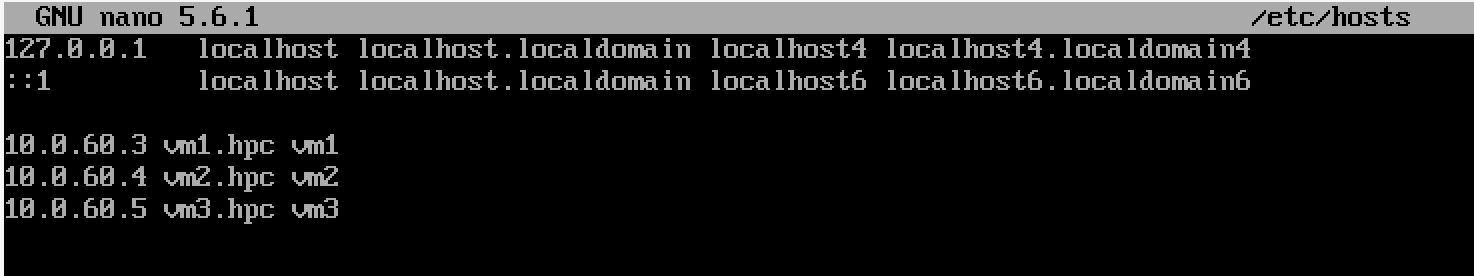
\includegraphics[width=0.7\linewidth]{img/4.png}
	\caption{Файл /etc/hosts с соответствием имен узлов}
	\label{fig:hosts}
\end{figure}

Для проверки связи между узлами необходимо воспользоваться командой {\bf ping remotehost}    ~\ref{fig:ping} :
\begin{figure}[h]
	\centering
	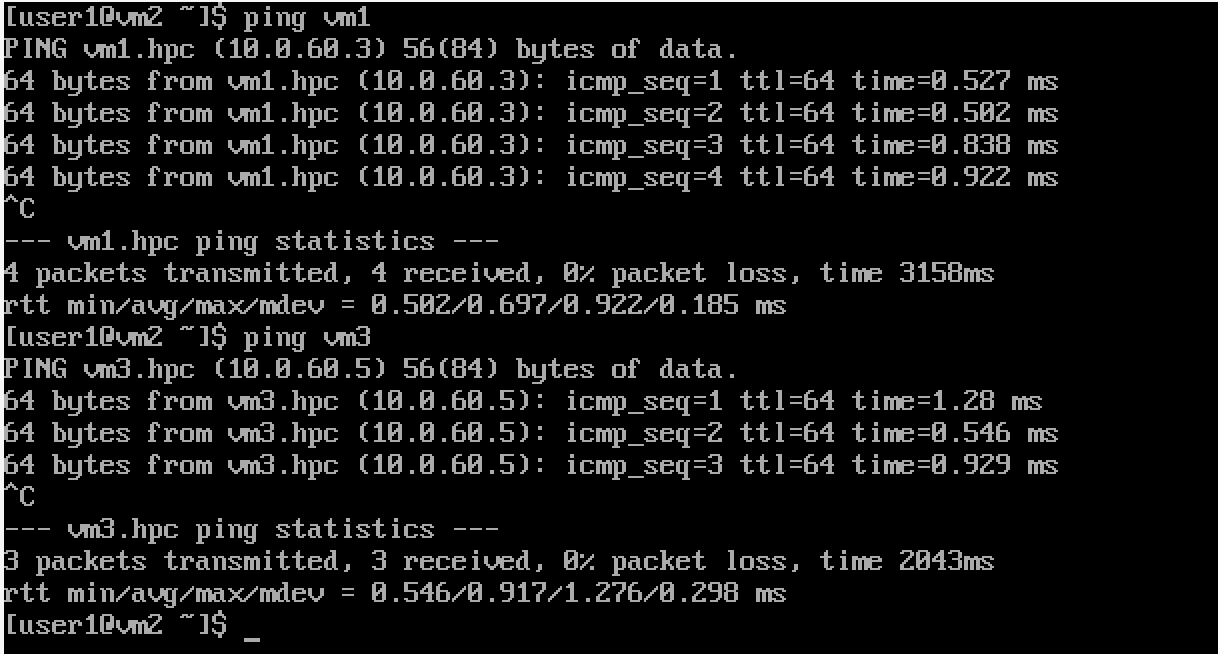
\includegraphics[width=0.7\linewidth]{img/5.png}
	\caption{Проверка связи между узлами}
	\label{fig:ping}
\end{figure}
\subsubsection{Настройка подключения по SSH}
SSH (Secure Shell) - это протокол для безопасного удаленного доступа к другим компьютерам в сети. \\ \newline
При настройки ОС в качестве дополнительного ПО SSH-сервер уже был установлен на каждой из виртуальных машин. Статус службы можно проверить командой {\bf sudo systemstl status ssh}. Служба должна быть запущена(active(running), но если это не так, то ее нужно запустить командой {\bf sudo systemctl start ssh}. \\ \newline
При стандартной авторизации по SSH пароль передается в незашифрованном
виде по сети, что может быть опасным для безопасности. Вместо этого, для
авторизации можно использовать ключи. Ключи - это пара файлов: закрытый ключ (private key) и открытый ключ (public key), которые используются
для проверки подлинности пользователя. \\ \newline
Для генерации ключевой пары на каждом узле необходимо выполнить: {\bf ssh-keygen -t rsa -b 4096 -f ~/.ssh/id\_rsa -N ""}. По умолчанию ключевая пара будет сохранена в каталоге /.ssh/.
Во время генерации ключевой пары можно задать пароль для закрытого
ключа. В данной работе пароль для закрытого ключа не установливался. \\ \newline
Открытый ключ должен быть размещен на удаленных узлах, к которым нужно подключиться без ввода пароля. Для этого можно воспользоваться командой {\bf ssh-copy-id user@remotehost}, где user - имя пользователя на удаленном хосте, а remotehost - адрес удаленного хоста, на который необходимо подключиться.
Если имена пользователей одинаковые, как в данной работе, можно указывать только адрес или доменное имя указанное раннее в файле hosts ({\bf ssh-copy-id remotehost}).
\begin{center}
	{\bf ssh-copy-id user1@vm1}\\ \vspace{7pt}
	{\bf ssh-copy-id vm2} 
\end{center}
После успешного выполнения команд при попытке подключения к удаленному хосту с помощью SSH не нужно будет вводить пароль. Чтобы проверить настройку ssh, можно подключиться с одной машины на другую с помощью команды {\bf ssh remotehost}. Если удалось подключиться без ввода пароля, то все настроено верно ~\ref{fig:ssh}.
\begin{figure}[h]
	\centering
	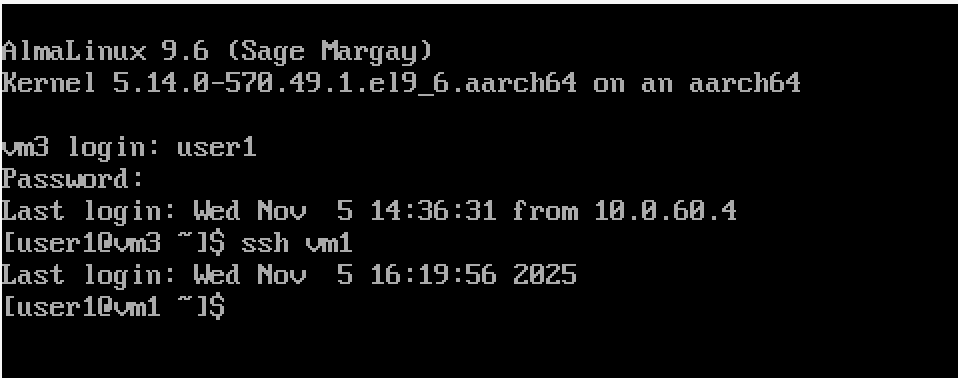
\includegraphics[width=0.7\linewidth]{img/6.png}
	\caption{Подключение по SSH}
	\label{fig:ssh}
\end{figure}
\subsubsection{Настройка буфера обмена с внешней системой}
Для того, чтобы была возможность пересылать файлы из основной ОС на виртуальные машины, необходимо настроить проброс портов сети NAT.  Для проброса портов необходимо перейти в панель «Инструменты», выбрать \text{«Сеть»}, затем \text{«Сети NAT»}. В качестве адреса хоста нужно указать 127.0.0.1(localhost) - стандартный локальный адрес. Если подключиться извне не получится, то localhost необходимо поменять на адрес сетевого адаптера VirtualBox(можно найти в параметрах основной системы). Порт хоста необходимо указать больше 4096, так как предыдущие порты являются привилегированными. Адрес гостя соответствует IP адресу виртуальной машины, а порт гостя по умолчанию 22 см. Рис. ~\ref{fig:port}.
\begin{figure}[h]
	\centering
	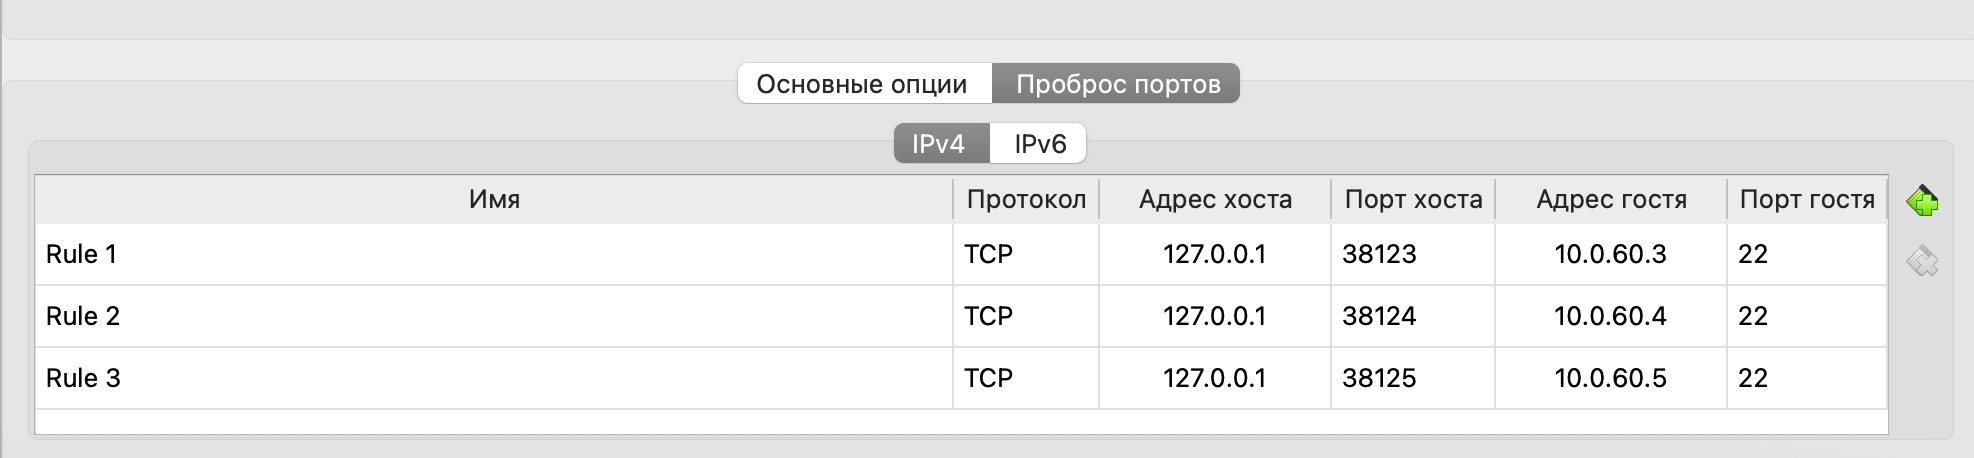
\includegraphics[width=0.7\linewidth]{img/7.png}
	\caption{Проброс портов}
	\label{fig:port}
\end{figure}

Если проброс портов выполнен верно, то получится зайти на виртуальную машину с командной строки основной системы. Для этого нужно ввести команду  {\bf ssh user@localhost -p port} и ввести пароль Рис. ~\ref{fig:win}.

\begin{figure}[h]
	\centering
	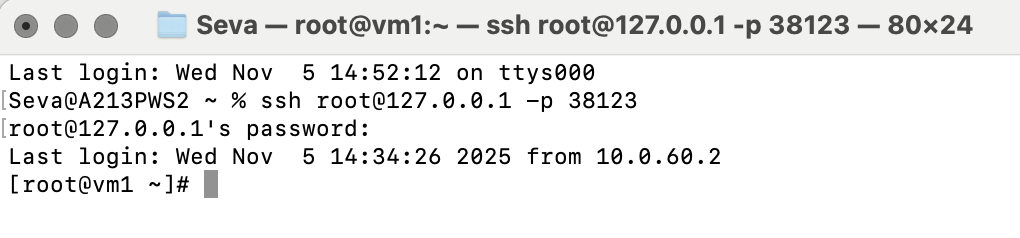
\includegraphics[width=0.7\linewidth]{img/10.png}
	\caption{Подключение с Терминала}
	\label{fig:win}
\end{figure}
Для отправки файлов с основной ОС на виртуальную необходимо использовать команду {\bf scp -P host\_port source\_path user@localhost:destination\_path}.
\subsection{Установка ПО для OpenMP. Тестовая программа.}
\begin{itemize}
	\item {\bf Определение OpenMP}  \\
	OpenMP (Open Multi-Processing) — это набор директив компилятора, библиотечных процедур и переменных окружения, которые предназначены для программирования многопоточных приложений на многопроцессорных системах с общей памятью. Официально поддерживается Си, С++ и Фортран, однако можно найти реализации для некоторых других языков, например Паскаль и Java. 
	\item {\bf Принцип работы OpenMP}  \\
	В стандарт OpenMP входят спецификации набора директив компилятора, вспомогательных функций и переменных среды. OpenMP реализует параллельные вычисления с помощью многопоточности, в которой «главный» (master) поток создает набор «подчиненных» (slave) потоков, и задача распределяется между ними.
	\item {\bf Основные возможности OpenMP:}
	\begin{enumerate}
		\item Директивы компилятора: OpenMP предоставляет специальные директивы, которые встраиваются в исходный код программы и указывают компилятору, какие участки кода должны выполняться параллельно. Например, директива \#pragma omp parallel создает команду для запуска параллельной секции кода.
		
		\itemРабота с потоками: OpenMP позволяет создавать потоки выполнения (threads) для распараллеливания работы. Потоки могут выполняться параллельно на многоядерном процессоре, ускоряя выполнение программы.
		
		\item Управление потоками: OpenMP предоставляет средства для управления потоками, такие как создание потоков, определение количества потоков, ограничение области видимости потоков и другие.
		
		\item Синхронизация: OpenMP предоставляет механизмы синхронизации потоков, такие как директивы \#pragma omp barrier для ожидания завершения работы всех потоков или \#pragma omp critical для создания критической секции.
		
		\item Распределение работы: OpenMP позволяет легко распределять работу между потоками с помощью директив, таких как \#pragma omp for, которая автоматически разбивает цикл на части и распределяет их между потоками.
	\end{enumerate}
\end{itemize}
Для установки OpenMP в AlmaLinux нужно воспользоваться пакетным менеджером apt, который используется для управления установкой, обновлением и удалением программ и пакетов:
\begin{enumerate}
	\item Установить компилятор g++, если его еще нет в системе:
	\begin{center}
		{\bf sudo dnf install gcc-c++}
	\end{center}
	Библиотека {\bf libgomp1} предоставляет поддержку OpenMP для компилятора GCC. Она содержит реализацию OpenMP API, необходимую для выполнения параллельных участков кода с использованием OpenMP.
	\item Установить пакеты, необходимые для разработки с поддержкой OpenMP:
	\begin{center}
		{\bf sudo dnf install gcc-c++ libomp-devel}
	\end{center}
\end{enumerate}
Для запуска программы с технологией OpenMP нужно:
\begin{enumerate}
	\item Создадим файл с расширением .сpp , напишем в нем простейшую программу \hyperref[1]{<<Листинг 1>>}.
	\label{1} \begin{lstlisting}[caption= Hello World] 
#include <omp.h>
#include <stdio.h>
#include <stdlib.h>

int main(int argc, char* argv[])
{
	#pragma omp parallel
	{
		printf("Hello World... from thread = %d\n",
		omp_get_thread_num());
	}
}
	\end{lstlisting}
	\item Скомпилируем файл, используя команду:
	\begin{center}
		{\bf mpicxx -fopenmp -o ttt ttt.cpp}
	\end{center}
	\item Установим число выполняемых одновременно потоков, используя переменную окружения:
	\begin{center}
		{\bf export OMP\_ NUM\_THREADS=N} - где N - кол-во потоков
	\end{center}
	\item Запустим исполняемый файл: 
	\begin{center}
		{\bf ./filename}
	\end{center}
	{\bf./filename} указывает путь к исполняемому файлу, который будет запущен на каждом из процессов. Важно, что {\bf ./} перед именем файла указывает, что
	файл находится в текущей директории.
	\item В результате работы программы выводится сообщение с номером потока 	Рис. ~\ref{fig:hi1}: 
 
	\begin{figure}[h]
		\centering
		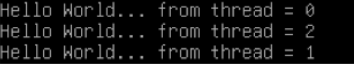
\includegraphics[width=0.7\linewidth]{img/8.png}
		\caption{Hello world для OpenMP}
		\label{fig:hi1}
	\end{figure}
\end{enumerate}
\subsection{Установка ПО для OpenMPI. Тестовая программа.}
\begin{itemize}
	\item {\bf Определение OpenMPI}  \\
	OpenMPI (Open Message Passing Interface) - это библиотека, предназначенная для разработки параллельных приложений, которая обеспечивает возможность обмена сообщениями между процессами, работающими на различных узлах вычислительного кластера.
	\item {\bf Принцип работы OpenMPI}  \\
	MPI-программа - это множество параллельных взаимодействующих процессов, которые работают каждый в своей выделенной области памяти. По сути это N независимых программ, которые общаются между собой в ходе работы.
	\item {\bf Основные возможности OpenMPI:} 
	\begin{enumerate}
		\item Механизмы передачи сообщений: OpenMPI предоставляет набор функций для отправки и приема сообщений между процессами, работающими на различных узлах кластера.
		\item Управление процессами: OpenMPI позволяет создавать, управлять и завершать параллельные процессы, а также устанавливать связи между ними.
		\item Поддержка различных архитектур: OpenMPI поддерживает работу на различных вычислительных архитектурах, включая кластеры с общей памятью (SMP), распределенные кластеры и другие.
		\item Гибкость конфигурации: OpenMPI обеспечивает гибкую настройку для различных типов сетей, протоколов передачи данных и других параметров, что делает его универсальным инструментом для разработки параллельных приложений.
	\end{enumerate}
\end{itemize}
Для установки OpenMPI в AlmaLinux нужно:
\begin{enumerate}
	\item Установить компилятор g++, если его еще нет в системе:
	\begin{center}
		{\bf sudo dnf install gcc-c++}
	\end{center}
	\item Установить пакеты, необходимые для разработки с поддержкой OpenMPI:
	\begin{center}
		{\bf sudo dnf install openmpi-devel}
	\end{center}
	{\bf libopenmpi3:} это название пакета библиотеки OpenMPI версии 3, который представляет собой реализацию стандарта сообщений MPI для создания параллельных приложений. \\
	
	{\bf libopenmpi-dev:} это название пакета, содержащего заголовочные файлы и статические библиотеки для разработки приложений, использующих библиотеку OpenMPI.
\end{enumerate}
Для запуска программы с технологией OpenMPI нужно:
\begin{enumerate}
	\item Создадим файл с расширением .сpp , напишем в нем простейшую программу \hyperref[1]{<<Листинг 2>>}.
	\label{2} \begin{lstlisting}[caption= Hello World] 
#include <iostream>
#include "mpi.h"
int main(int argc, char **argv) {
	int AMOUNT_FLOW, RANK_NUMBER;
	MPI_Init(&argc, &argv);
	MPI_Comm_size(MPI_COMM_WORLD, &AMOUNT_FLOW);
	MPI_Comm_rank(MPI_COMM_WORLD, &RANK_NUMBER);
	std::cout << " Hello, World! From "
	<< RANK_NUMBER << " process" << std::endl;
	MPI_Finalize();
	return 0;
}
	\end{lstlisting}
	\item Скомпилируем файл, используя команду:
	\begin{center}
		{\bf mpicc -o ttt ttt.c}
	\end{center}
	\item Запустим исполняемый файл(пример): 
	\begin{center}
		{\bf mpirun -host vm1 -np 1 ./ttt : -host vm2 -np 1 ./ttt : -host vm3 -np 1 ./ttt}
	\end{center}
	Эта команда запустит программу filename с 7 процессами на трех узлах vm1, vm2 и vm3. При этом важно не забывать, что код программы должен быть одинаковым на каждом узле, и компиляция файла с помощью команды mpic++ должна быть произведена на каждом из узлов.
	\item В результате работы программы выводится сообщение с номером процесса Рис. ~\ref{fig:hi2} : 
\end{enumerate}
\begin{figure}[h]
	\centering
	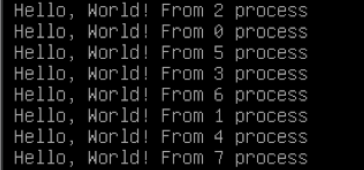
\includegraphics[width=0.7\linewidth]{img/9.png}
	\caption{Hello world для OpenMPI}
	\label{fig:hi2}
\end{figure}

\newpage
\section{Реализация параллельного программирования с использованием OpenMP и OpenMPI}

\subsection{Технология OpenMP}

Для реализации многопоточных вычислений на одном узле была использована технология OpenMP. Основные директивы, примененные в работе:

\textbf{Параллельные регионы:}
\begin{lstlisting}[caption=Параллельное вычисление степеней вершин, label=lst:vertex_degrees, language=C++]
	#pragma omp parallel for
	for (int i = 0; i < n; ++i) {
		int degree = 0;
		for (int j = 0; j < n; ++j) {
			if (matrix_Of_Adjacency_Unoriented[i][j] != 0) { degree++; }
		}
		nodesDegree[i] = degree;
	}
\end{lstlisting}

\textbf{Распараллеливание вложенных циклов:}
\begin{lstlisting}[caption=Параллельное заполнение матрицы весов, label=lst:weight_matrix, language=C++]
	#pragma omp parallel for collapse(2)
	for (int i = 0; i < nodes; ++i) {
		for (int j = 0; j < nodes; ++j) {
			if (matrix_Of_Adjacency[i][j] == 1) {
				int weight = getRandomWeight(2);
				matrix_Of_Weights_Unoriented[i][j] = weight;
				matrix_Of_Weights_Unoriented[j][i] = weight;
			}
		}
	}
\end{lstlisting}

\textbf{Критические секции:}
\begin{lstlisting}[caption=Безопасное добавление рёбер в общий вектор, label=lst:critical_section, language=C++]
	#pragma omp critical
	{
		edges.push_back(Edge(u, v, weight));
	}
\end{lstlisting}

\newpage
\textbf{Редукционные операции:}
\begin{lstlisting}[caption=Вычисление общего веса минимального остова, label=lst:mst_weight, language=C++]
	#pragma omp parallel for reduction(+:totalWeight)
	for (int i = 0; i < nodes; ++i) {
		for (int j = 0; j < nodes; ++j) {
			if (mst[i][j] != 0) {
				totalWeight += mst[i][j];
			}
		}
	}
\end{lstlisting}

\subsection{Технология OpenMPI}

Для распределенных вычислений на нескольких узлах кластера была использована технология OpenMPI. Функции, примененные в работе:

\textbf{Инициализация MPI:}
\begin{lstlisting}[caption=Инициализация MPI окружения, label=lst:mpi_init, language=C++]
	MPI_Init(&argc, &argv);
	MPI_Comm_rank(MPI_COMM_WORLD, &world_rank);
	MPI_Comm_size(MPI_COMM_WORLD, &world_size);
\end{lstlisting}

\textbf{Широковещательная рассылка данных:}
\begin{lstlisting}[caption=Рассылка параметров графа, label=lst:mpi_bcast, language=C++]
	MPI_Bcast(&nodes, 1, MPI_INT, 0, MPI_COMM_WORLD);
	MPI_Bcast(&chose, 1, MPI_INT, 0, MPI_COMM_WORLD);
\end{lstlisting}

\textbf{Глобальная редукция:}
\begin{lstlisting}[caption=Синхронизация матриц между процессами, label=lst:mpi_allreduce, language=C++]
	MPI_Allreduce(MPI_IN_PLACE, matrix_Of_Adjacency[i].data(), 
	nodes, MPI_INT, MPI_MAX, MPI_COMM_WORLD);
	MPI_Allreduce(&localWeight, &totalWeight, 1, 
	MPI_INT, MPI_SUM, MPI_COMM_WORLD);
\end{lstlisting}

\textbf{Передача данных между процессами:}
\begin{lstlisting}[caption=Сбор данных о степенях вершин, label=lst:mpi_send_recv, language=C++]
	MPI_Send(nodesDegree.data() + start, end - start, 
	MPI_INT, 0, 0, MPI_COMM_WORLD);
	
	MPI_Recv(nodesDegree.data() + recv_start, 
	recv_end - recv_start, MPI_INT, i, 0, 
	MPI_COMM_WORLD, MPI_STATUS_IGNORE);
\end{lstlisting}

\subsection{Гибридный подход OpenMP + OpenMPI}

Был реализован гибридный подход, сочетающий преимущества обеих технологий:

\begin{lstlisting}[caption=Гибридная генерация графа, label=lst:hybrid_graph_gen, language=C++]
	void generateGraphDistributed(bool allowNegativeWeights, int world_rank, int world_size) {
		std::random_device rd;
		std::mt19937 gen(rd());
		int minW = allowNegativeWeights ? -10 : 1;
		std::uniform_int_distribution<int> dist(minW, 10);
		
		int n = getRows();
		int chunk_size = n / world_size;
		int start = world_rank * chunk_size;
		int end = (world_rank == world_size - 1) ? n : start + chunk_size;
		
		#pragma omp parallel for collapse(2)
		for (int i = start; i < end; ++i) {
			for (int j = 0; j < n; ++j) {
				if (i != j) {
					#pragma omp critical
					set(i, j, dist(gen));
				}
			}
		}
		syncMatrixAcrossProcesses();
	}
\end{lstlisting}

\subsection{Вспомогательная функция синхронизации матриц}

Для  согласованной работы данных между процессами была реализована вспомогательная функция синхронизации матриц. Данная функция является критически важной компонентой распределенной системы, обеспечивающей целостность данных при работе в многопроцессорной среде. 
\par Функция \texttt{syncMatrixAcrossProcesses()} выполняет следующие ключевые задачи:

\begin{itemize}
	\item \textbf{Сериализация данных}: Преобразует двумерную матрицу в одномерный массив для эффективной передачи через сеть
	\item \textbf{Глобальная синхронизация}: Использует операцию \texttt{MPI\_Allreduce} с операцией \texttt{MPI\_MAX} для объединения данных со всех процессов
	\item \textbf{Восстановление структуры}: Преобразует синхронизированный плоский массив обратно в двумерную матрицу
\end{itemize}

\begin{lstlisting}[caption=Функция синхронизации матриц между процессами, label=lst:matrix_sync, language=C++]
	void syncMatrixAcrossProcesses() {
		int n = getRows();
		std::vector<int> flatMatrix(n * n);
		for (int i = 0; i < n; ++i) {
			for (int j = 0; j < n; ++j) {
				flatMatrix[i * n + j] = get(i, j);
			}
		}
		MPI_Allreduce(MPI_IN_PLACE, flatMatrix.data(), n * n, 
		MPI_INT, MPI_MAX, MPI_COMM_WORLD);
		for (int i = 0; i < n; ++i) {
			for (int j = 0; j < n; ++j) {
				set(i, j, flatMatrix[i * n + j]);
			}
		}
	}
\end{lstlisting}

\subsection{Управление параллельным выполнением}

\textbf{Синхронизация процессов}
\begin{lstlisting}[caption=Барьерная синхронизация процессов, label=lst:mpi_barrier, language=C++]
	MPI_Barrier(MPI_COMM_WORLD);
\end{lstlisting}

\textbf{Завершение работы}
\begin{lstlisting}[caption=Корректное завершение MPI, label=lst:mpi_finalize, language=C++]
	MPI_Finalize();
\end{lstlisting}

\textbf{Управление потоками}
\begin{lstlisting}[caption=Настройка количества потоков OpenMP, label=lst:omp_threads, language=C++]
	omp_set_num_threads(2);
\end{lstlisting}

\newpage
\section{Распараллеливание алгоритмов в программе}

В рамках данной работы была проведена комплексная работа по распараллеливанию основных алгоритмов теории графов с использованием технологий OpenMP и OpenMPI. Каждый алгоритм был адаптирован для работы в многопроцессорной и распределенной среде с учетом его специфических особенностей.

\textbf{Генерация графа: \texttt{void generateGraphDistributed(bool allowNegativeWeights, int world\_rank, int world\_size)}}

Для создания графов больших размеров был реализован распределенный алгоритм генерации, сочетающий подходы OpenMP и OpenMPI. Процесс с рангом 0 выполняет роль координатора, распределяя работу между всеми узлами кластера. Каждый процесс генерирует свою порцию вершин и рёбер, используя многопоточность OpenMP для внутреннего распараллеливания. Для обеспечения согласованности данных применяется синхронизация матриц смежности через операцию MPI\_Allreduce, что гарантирует идентичность представления графа на всех узлах вычислительной системы.

\textbf{Алгоритм Беллмана-Форда: \texttt{BellmanFordResult bellmanFordDistributed(int source, int world\_rank, int world\_size) const}}

Распараллеливание алгоритма поиска кратчайших путей в ориентированных графах с возможными отрицательными весами было реализовано с использованием гибридного подхода. Вычисления распределяются между MPI-процессами, каждый из которых обрабатывает свою часть вершин графа. Внутри каждого процесса применяется OpenMP для параллельного обновления расстояний до соседних вершин. Особое внимание уделено обработке отрицательных циклов — их обнаружение также выполняется параллельно с последующей синхронизацией результатов между всеми процессами.

\textbf{Алгоритм Крускала: \texttt{MSTResult kruskalMSTDistributed(int world\_rank, int world\_size) const}}

Построение минимального остовного дерева было распараллелено за счет распределенного сбора и сортировки рёбер графа. Каждый процесс анализирует своё подмножество рёбер, используя многопоточность OpenMP для эффективного перебора возможных соединений. Собранные рёбра передаются на главный процесс, где выполняется их сортировка по весу и построение MST с использованием системы непересекающихся множеств. Вычисление общего веса минимального остова осуществляется через операцию MPI\_Allreduce, обеспечивая получение корректного результата на всех узлах.

\textbf{Алгоритм Борувки: \texttt{vector<UndirectedGraph::Edge> boruvkaMSTDistributed(const UndirectedGraph\& graph, int world\_rank, int world\_size)}}

Альтернативный алгоритм построения минимального остовного дерева был реализован с акцентом на распределенную обработку компонент связности. Каждый процесс независимо обрабатывает назначенные ему рёбра, определяя минимальные исходящие соединения для своих компонент. Результаты локальных вычислений собираются на главном процессе, где выполняется объединение компонент и формирование итогового остовного дерева. Подход особенно эффективен для разреженных графов больших размеров.

\textbf{Обход в ширину (BFS): \texttt{vector<int> bfsTraversalDistributed(const DirectedGraph\& graph, int start, int world\_rank, int world\_size)}}

Распределенная версия алгоритма обхода в ширину реализована с использованием динамического распределения вершин между процессами. На каждой итерации текущий фронт обхода распределяется между всеми узлами кластера, что позволяет эффективно обрабатывать графы с большим диаметром. Применение OpenMP внутри каждого процесса ускоряет обработку соседей текущих вершин, а механизмы MPI-коммуникации обеспечивают согласованность информации о посещенных вершинах.

\textbf{Раскраска графа: \texttt{ColoringResult greedyColoringDistributed(int world\_rank, int world\_size) const}}

Жадный алгоритм раскраски графа был адаптирован для распределенного выполнения через итеративную синхронизацию цветов между процессами. Каждый узел обрабатывает свою порцию вершин, выбирая минимальный доступный цвет на основе информации о раскраске соседних вершин. После каждой итерации выполняется обмен информацией о новых цветах через MPI\_Allreduce, что гарантирует корректность раскраски и предотвращает конфликты между процессами.

\newpage
\section{Результаты работы}

\subsection{Тестирование OpenMP}

Программа была протестирована с использованием технологии OpenMP от двух пользователей user1 (user1234) и root(12345678). Успешно выполнены:
\begin{itemize}
	\item Параллельная генерация графов
	\item Параллельный алгоритм Беллмана-Форда
	\item Параллельный алгоритм Крускала
	\item Параллельная раскраска графов
	\item Параллельный обход в ширину
\end{itemize}

\begin{figure}[h]
	\centering
	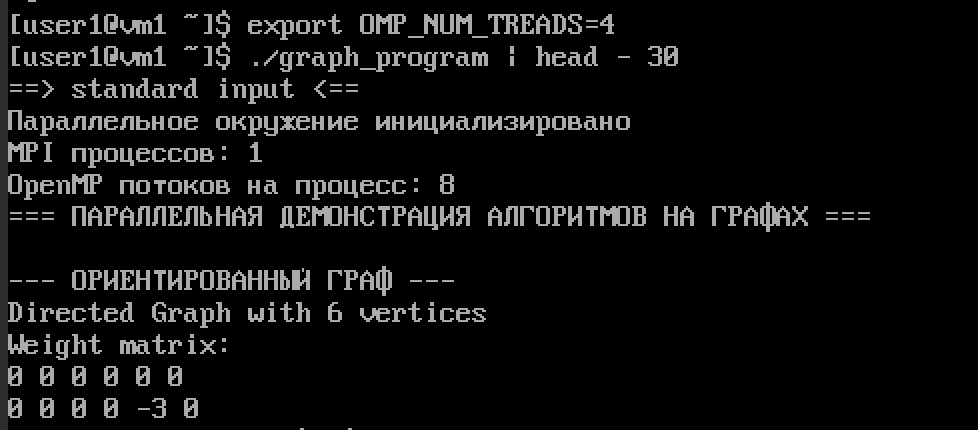
\includegraphics[width=0.7\linewidth]{img/2.png}
	\caption{Результаты работы OpenMP}
	\label{fig:omp_results}
\end{figure}

\subsection{Тестирование MPI}

Программа была запущена на трех виртуальных машинах с использованием MPI. Доказана работоспособность распределенных вычислений.

\begin{figure}[h]
	\centering
	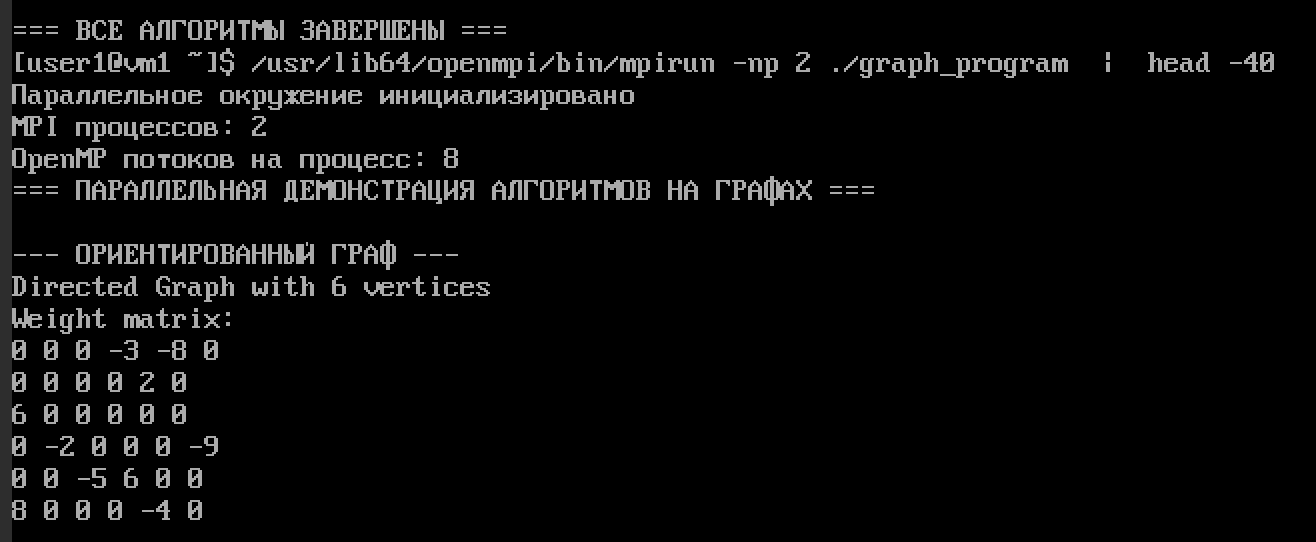
\includegraphics[width=0.7\linewidth]{img/3.png}
	\caption{Результаты работы MPI}
	\label{fig:mpi_results}
\end{figure}

\newpage
\subsection{Сравнение производительности}

Было проведено сравнение времени выполнения алгоритмов на различном количестве потоков и процессов.

\begin{table}[h]
	\centering
	\begin{tabular}{|c|c|c|c|}
		\hline
		Алгоритм & 3 процесса и 8 потоков & 3 процесса и 2 потока & 1 процесс и 8 потоков \\
		\hline
		Обход в ширину & 15.0547мс & 48.1351мс  & 0.298921мс  \\
		\hline
		Беллман-Форд & 48.6687мс & 12.7087мс  & 0.479755мс  \\
		\hline
		Крускал & 0.654147мс & 0.537119мс  & 0.023338мс  \\
		\hline
		Борувки & 0.007751мс & 0.673877мс  & 0.006591мс  \\
		\hline
		Раскраска & 8.69731мс & 9.80072мс  & 0.078274мс  \\
		\hline
		Эйлеровы свойства & 0.173903мс & 0.111046мс  & 0.298921мс  \\
		\hline
		Фано & 0.14127мс & 0.014334мс  & 0.012143мс  \\
		\hline
	\end{tabular}
	\caption{Сравнение времени выполнения алгоритмов}
	\label{tab:performance}
\end{table}

Данные из таблицы показывают, что с увелечением потоков растет производительность. А также видно, что при малых значениях, распараллеливание на процессы приводит к ухудшению результата. При повышении сложностей алгоритмов, производительность многопроцессорности будет также расти.

\newpage
\section*{ЗАКЛЮЧЕНИЕ}
\addcontentsline{toc}{section}{ЗАКЛЮЧЕНИЕ}

В ходе выполнения научно-исследовательской работы были изучены и применены методы параллельного программирования с использованием технологий OpenMP и MPI. Реализовано приложение на языке C++, настроена сеть виртуальных машин для запуска распределённых вычислений.

Созданы 3 виртуальные машины, изучены основы взаимодействия с ОС Linux на примере AlmaLinux. Реализованы параллельные версии алгоритмов теории графов:
\begin{itemize}
	\item подсчёт количества остовных деревьев;
	\item поиск минимального остова по алгоритму Краскла;
	\item алгоритм Беллмана-Форда для поиска кратчайших путей;
	\item жадная раскраска графа;
	\item обход графа в ширину.
\end{itemize}

Все алгоритмы успешно распараллелены с использованием технологий OpenMP и MPI. Доказана работоспособность распределенной системы из трех виртуальных машин.

Оценка полноты решений поставленных задач: все поставленные задачи выполнены в полном объеме. Разработаны рекомендации по использованию результатов работы в учебном процессе для демонстрации принципов параллельного программирования.

Результаты оценки научно-технического уровня: работа соответствует современному уровню развития технологий параллельного программирования и может быть использована в образовательных целях.

Полученные навыки и опыт могут послужить хорошей практической основой для дальнейшего углубления в изучение суперкомпьютерных технологий и высокопроизводительных вычислений.

\newpage
\section*{СПИСОК ИСПОЛЬЗОВАННЫХ ИСТОЧНИКОВ}
\addcontentsline{toc}{section}{СПИСОК ИСПОЛЬЗОВАННЫХ ИСТОЧНИКОВ}

\begin{enumerate}
	\item Секция «Телематика». — Текст : электронный // tema.spbstu.ru : [сайт]. — URL: https://tema.spbstu.ru/tgraph/ (дата обращения: 29.06.2025).
	\item The Slackware Linux Project. — Текст : электронный // slackware.com : [сайт]. — URL: http://www.slackware.com/ (дата обращения: 20.06.2025).
	\item OpenMPI [Электронный ресурс] / Lawrence Livermore National Laboratory. — Режим доступа: https://hpc-tutorials.llnl.gov/mpi/ (дата обращения: 28.06.2025).
	\item OpenMP [Электронный ресурс] / Lawrence Livermore National Laboratory. — Режим доступа: https://hpc-tutorials.llnl.gov/openmp/ (дата обращения: 28.06.2025).
	\item MPI: A Message-Passing Interface Standard. Version 3.1. — High Performance Computing Center Stuttgart, 2015. — 866 с.
	\item OpenMP Application Program Interface. Version 5.0. — OpenMP Architecture Review Board, 2020. — 530 с.
	\item Форсайт Дж., Малькольм М., Моулер К. Машинные методы математических вычислений. — М.: Мир, 1980. — 280 с.
\end{enumerate}

\newpage
\section*{ПРИЛОЖЕНИЕ А}
\addcontentsline{toc}{section}{ПРИЛОЖЕНИЕ А}

\textbf{Исходный код программы}
	
	\begin{lstlisting}[caption=Основной файл программы, label=lst:main, language=C++]
#include <iostream>
#include <vector>
#include <queue>
#include <climits>
#include <algorithm>
#include <set>
#include <functional>
#include <random>
#include <stdexcept>
#include <map>
#include <stack>
#include <list>
#include <omp.h>
#include <mpi.h>
#include <numeric>

using namespace std;

const int MAX_OMP_THREADS = 8;
const int ROOT_RANK = 0;

class Matrix {
protected:
std::vector<std::vector<int>> data;
int rows, cols;

public:
Matrix(int r, int c) : rows(r), cols(c) {
data.resize(rows, std::vector<int>(cols, 0));
}

virtual ~Matrix() = default;

int getRows() const { return rows; }
int getCols() const { return cols; }

int get(int row, int col) const {
if (row >= 0 && row < rows && col >= 0 && col < cols) {
return data[row][col];
}
throw std::out_of_range("Invalid index");
}

void set(int row, int col, int value) {
if (row >= 0 && row < rows && col >= 0 && col < cols) {
data[row][col] = value;
} else {
throw std::out_of_range("Invalid index");
}
}

void print() const {
for (int i = 0; i < rows; ++i) {
for (int j = 0; j < cols; ++j) {
std::cout << data[i][j] << " ";
}
std::cout << std::endl;
}
}

void printWeightMatrix() const {
std::cout << "Weight matrix:\n";
print();
}
};

class Graph : public Matrix {
public:
Graph(int vertices) : Matrix(vertices, vertices) {}

virtual void generateGraph(bool allowNegativeWeights) = 0;
virtual void printInfo() const = 0;
};

class DirectedGraph : public Graph {
private:
void syncMatrixAcrossProcesses() {
int n = getRows();
std::vector<int> flatMatrix(n * n);

for (int i = 0; i < n; ++i) {
for (int j = 0; j < n; ++j) {
flatMatrix[i * n + j] = get(i, j);
}
}

MPI_Allreduce(MPI_IN_PLACE, flatMatrix.data(), n * n, MPI_INT, MPI_MAX, MPI_COMM_WORLD);

for (int i = 0; i < n; ++i) {
for (int j = 0; j < n; ++j) {
set(i, j, flatMatrix[i * n + j]);
}
}
}

public:
DirectedGraph(int vertices) : Graph(vertices) {}
void generateGraph(bool allowNegativeWeights) override {
std::random_device rd;
std::mt19937 gen(rd());
int minW = allowNegativeWeights ? -10 : 1;
std::uniform_int_distribution<int> dist(minW, 10);

#pragma omp parallel for collapse(2)
for (int i = 0; i < getRows(); ++i) {
for (int j = 0; j < getCols(); ++j) {
if (i != j && dist(gen) > 5) {
#pragma omp critical
set(i, j, dist(gen));
}
}
}
}

void generateGraphDistributed(bool allowNegativeWeights, int world_rank, int world_size) {
std::random_device rd;
std::mt19937 gen(rd());
int minW = allowNegativeWeights ? -10 : 1;
std::uniform_int_distribution<int> dist(minW, 10);

int n = getRows();
int chunk_size = n / world_size;
int start = world_rank * chunk_size;
int end = (world_rank == world_size - 1) ? n : start + chunk_size;

#pragma omp parallel for collapse(2)
for (int i = start; i < end; ++i) {
for (int j = 0; j < n; ++j) {
if (i != j) {
#pragma omp critical
set(i, j, dist(gen));
}
}
}

syncMatrixAcrossProcesses();
}

void printInfo() const override {
std::cout << "Directed Graph with " << getRows() << " vertices\n";
printWeightMatrix();
}

struct BellmanFordResult {
bool hasNegativeCycle;
int iterations;
std::vector<int> distances;
std::vector<int> predecessors;
};

BellmanFordResult bellmanFord(int source) const {
int n = getRows();
BellmanFordResult result;
result.iterations = 0;
result.distances.assign(n, INT_MAX);
result.predecessors.assign(n, -1);
result.hasNegativeCycle = false;
result.distances[source] = 0;

for (int i = 0; i < n - 1; ++i) {
bool updated = false;

#pragma omp parallel for reduction(||:updated)
for (int u = 0; u < n; ++u) {
if (result.distances[u] == INT_MAX) continue;

for (int v = 0; v < n; ++v) {
int weight = get(u, v);
if (weight != 0 && result.distances[u] != INT_MAX) {
if (result.distances[v] > result.distances[u] + weight) {
#pragma omp critical
{
result.distances[v] = result.distances[u] + weight;
result.predecessors[v] = u;
updated = true;
}
}
}
}
}
result.iterations++;

if (!updated) break;
}

#pragma omp parallel for
for (int u = 0; u < n; ++u) {
if (result.distances[u] == INT_MAX) continue;

for (int v = 0; v < n; ++v) {
int weight = get(u, v);
if (weight != 0 && result.distances[u] != INT_MAX) {
if (result.distances[v] > result.distances[u] + weight) {
result.hasNegativeCycle = true;
result.distances[v] = INT_MIN;
}
}
}
}

return result;
}

BellmanFordResult bellmanFordDistributed(int source, int world_rank, int world_size) const {
int n = getRows();
BellmanFordResult result;
result.iterations = 0;
result.distances.assign(n, INT_MAX);
result.predecessors.assign(n, -1);
result.hasNegativeCycle = false;

if (world_rank == 0) {
result.distances[source] = 0;
}

MPI_Bcast(result.distances.data(), n, MPI_INT, 0, MPI_COMM_WORLD);
MPI_Bcast(result.predecessors.data(), n, MPI_INT, 0, MPI_COMM_WORLD);

int chunk_size = n / world_size;
int remainder = n % world_size;
int start = world_rank * chunk_size;
int end = (world_rank == world_size - 1) ? n : start + chunk_size;
int local_size = end - start;

for (int i = 0; i < n - 1; ++i) {
bool local_updated = false;
vector<int> local_distances = result.distances;
vector<int> local_predecessors = result.predecessors;

#pragma omp parallel for reduction(||:local_updated)
for (int u = 0; u < n; ++u) {
if (result.distances[u] == INT_MAX) continue;

for (int v = start; v < end; ++v) {
int weight = get(u, v);
if (weight != 0 && result.distances[u] != INT_MAX) {
long long new_dist = (long long)result.distances[u] + weight;
if (new_dist < INT_MAX && new_dist < result.distances[v]) {
#pragma omp critical
{
local_distances[v] = new_dist;
local_predecessors[v] = u;
local_updated = true;
}
}
}
}
}

vector<int> all_distances(n);

MPI_Allreduce(local_distances.data(), all_distances.data(), n, MPI_INT, MPI_MIN, MPI_COMM_WORLD);

for (int v = 0; v < n; ++v) {
if (all_distances[v] != result.distances[v]) {
result.distances[v] = all_distances[v];
result.predecessors[v] = local_predecessors[v];
}
}

int global_updated;
MPI_Allreduce(&local_updated, &global_updated, 1, MPI_INT, MPI_MAX, MPI_COMM_WORLD);

result.iterations++;

if (!global_updated) break;
}

bool local_negative_cycle = false;

#pragma omp parallel for reduction(||:local_negative_cycle)
for (int u = 0; u < n; ++u) {
if (result.distances[u] == INT_MAX) continue;

for (int v = start; v < end; ++v) {
int weight = get(u, v);
if (weight != 0 && result.distances[u] != INT_MAX) {
long long new_dist = (long long)result.distances[u] + weight;
if (new_dist < result.distances[v]) {
local_negative_cycle = true;
#pragma omp critical
{
result.distances[v] = INT_MIN;
}
}
}
}
}

int global_negative_cycle;
MPI_Allreduce(&local_negative_cycle, &global_negative_cycle, 1, MPI_INT, MPI_MAX, MPI_COMM_WORLD);
result.hasNegativeCycle = global_negative_cycle;

MPI_Allreduce(MPI_IN_PLACE, result.distances.data(), n, MPI_INT, MPI_MIN, MPI_COMM_WORLD);

return result;
}
};

class UndirectedGraph : public Graph {
public:
UndirectedGraph(int vertices) : Graph(vertices) {}
void generateGraph(bool allowNegativeWeights) override {
std::random_device rd;
std::mt19937 gen(rd());
int minW = allowNegativeWeights ? -10 : 1;
std::uniform_int_distribution<int> dist(minW, 10);

#pragma omp parallel for
for (int i = 0; i < getRows(); ++i) {
for (int j = i + 1; j < getCols(); ++j) {
if (dist(gen) > 5) {
int weight = dist(gen);
#pragma omp critical
{
set(i, j, weight);
set(j, i, weight);
}
}
}
}
}

void generateGraphDistributed(bool allowNegativeWeights, int world_rank, int world_size) {
std::random_device rd;
std::mt19937 gen(rd() + world_rank);

int n = getRows();
int chunk_size = n / world_size;
int remainder = n % world_size;
int start = world_rank * chunk_size + std::min(world_rank, remainder);
int end = start + chunk_size + (world_rank < remainder ? 1 : 0);

for (int i = start; i < end; ++i) {
for (int j = i + 1; j < n; ++j) {
double prob = static_cast<double>(gen() % 100) / 100.0;
if (prob > 0.3) {
int weight;
do {
weight = (allowNegativeWeights ? (gen() % 21 - 10) : (gen() % 10 + 1));
} while (weight == 0);

set(i, j, weight);
set(j, i, weight);
}
}
}

syncMatrixUndirected(world_rank, world_size);
}


void printInfo() const override {
std::cout << "Undirected Graph with " << getRows() << " vertices\n";
printWeightMatrix();
}

void addEdge(int from, int to, int weight) {
set(from, to, weight);
set(to, from, weight);
}

struct Edge {
int u, v, weight;
Edge() : u(0), v(0), weight(0) {}
Edge(int u, int v, int w) : u(u), v(v), weight(w) {}
bool operator<(const Edge& other) const {
return weight < other.weight;
}
};

struct MSTResult {
std::vector<Edge> edges;
int totalWeight = 0;
bool success = false;
std::string message;
};

class DSU {
public:
std::vector<int> parent, rank;

DSU(int n) {
parent.resize(n);
rank.resize(n, 0);
#pragma omp parallel for
for (int i = 0; i < n; i++) parent[i] = i;
}

int find(int x) {
if (parent[x] != x) {
parent[x] = find(parent[x]);
}
return parent[x];
}

void unite(int x, int y) {
int rootX = find(x);
int rootY = find(y);

if (rootX != rootY) {
if (rank[rootX] < rank[rootY]) {
parent[rootX] = rootY;
} else if (rank[rootX] > rank[rootY]) {
parent[rootY] = rootX;
} else {
parent[rootY] = rootX;
rank[rootX]++;
}
}
}
};


MSTResult kruskalMST() const {
MSTResult result;
int n = getRows();

std::vector<Edge> edges;
#pragma omp parallel for collapse(2)
for (int i = 0; i < n; i++) {
for (int j = i + 1; j < n; j++) {
int weight = get(i, j);
if (weight != 0) {
#pragma omp critical
edges.push_back(Edge(i, j, weight));
}
}
}

#pragma omp parallel
{
#pragma omp single
std::sort(edges.begin(), edges.end());
}

DSU dsu(n);
result.totalWeight = 0;
int edgesUsed = 0;

int local_totalWeight = 0;
int local_edgesUsed = 0;
#pragma omp parallel for reduction(+:local_totalWeight, local_edgesUsed)
for (size_t i = 0; i < edges.size(); i++) {
const Edge& edge = edges[i];
if (dsu.find(edge.u) != dsu.find(edge.v)) {
#pragma omp critical
{
if (dsu.find(edge.u) != dsu.find(edge.v)) {
result.edges.push_back(edge);
local_totalWeight += edge.weight;
dsu.unite(edge.u, edge.v);
local_edgesUsed++;
}
}
}
}
result.totalWeight = local_totalWeight;
edgesUsed = local_edgesUsed;

if (edgesUsed == n - 1) {
result.success = true;
} else {
result.success = false;
}

return result;
}

MSTResult kruskalMSTDistributed(int world_rank, int world_size) const {

MSTResult result;
int n = getRows();

std::vector<Edge> local_edges;

#pragma omp parallel
{
std::vector<Edge> private_edges;

#pragma omp for collapse(2) nowait
for (int i = world_rank; i < n; i += world_size) {
for (int j = i + 1; j < n; j++) {
int weight = get(i, j);
if (weight != 0) {
private_edges.push_back(Edge(i, j, weight));
}
}
}

#pragma omp critical
local_edges.insert(local_edges.end(), private_edges.begin(), private_edges.end());
}

#pragma omp parallel
{
#pragma omp single
std::sort(local_edges.begin(), local_edges.end());
}

if (world_rank == ROOT_RANK) {
std::vector<Edge> all_edges = local_edges;

for (int i = 1; i < world_size; i++) {
int edge_count;
MPI_Recv(&edge_count, 1, MPI_INT, i, 0, MPI_COMM_WORLD, MPI_STATUS_IGNORE);

std::vector<Edge> temp_edges(edge_count);
MPI_Recv(temp_edges.data(), edge_count * 3, MPI_INT, i, 1, MPI_COMM_WORLD, MPI_STATUS_IGNORE);

all_edges.insert(all_edges.end(), temp_edges.begin(), temp_edges.end());
}

#pragma omp parallel
{
#pragma omp single
std::sort(all_edges.begin(), all_edges.end());
}

DSU dsu(n);
result.totalWeight = 0;
int edgesUsed = 0;

std::vector<Edge> mst_edges;
mst_edges.reserve(n - 1);


#pragma omp parallel
{
DSU local_dsu = dsu;
std::vector<Edge> local_mst;
int local_weight = 0;
int local_count = 0;

#pragma omp for schedule(static)
for (size_t i = 0; i < all_edges.size(); i++) {
if (local_count >= n - 1) continue;

const Edge& edge = all_edges[i];
if (local_dsu.find(edge.u) != local_dsu.find(edge.v)) {
local_mst.push_back(edge);
local_weight += edge.weight;
local_dsu.unite(edge.u, edge.v);
local_count++;
}
}

#pragma omp critical
{
for (const Edge& edge : local_mst) {
if (dsu.find(edge.u) != dsu.find(edge.v)) {
mst_edges.push_back(edge);
result.totalWeight += edge.weight;
dsu.unite(edge.u, edge.v);
edgesUsed++;
}
}
}
}

result.edges = mst_edges;
result.success = (edgesUsed == n - 1);
result.message = result.success ? 0 : 1;

} else {
int edge_count = local_edges.size();
MPI_Send(&edge_count, 1, MPI_INT, ROOT_RANK, 0, MPI_COMM_WORLD);

if (edge_count > 0) {
std::vector<int> edge_data;
edge_data.reserve(edge_count * 3);

#pragma omp parallel for
for (int i = 0; i < edge_count; i++) {
const Edge& edge = local_edges[i];
#pragma omp critical
{
edge_data.push_back(edge.u);
edge_data.push_back(edge.v);
edge_data.push_back(edge.weight);
}
}

MPI_Send(edge_data.data(), edge_count * 3, MPI_INT, ROOT_RANK, 1, MPI_COMM_WORLD);
}
}

if (world_size > 1) {
int success_int = result.success ? 1 : 0;
MPI_Bcast(&success_int, 1, MPI_INT, ROOT_RANK, MPI_COMM_WORLD);
result.success = (success_int == 1);

MPI_Bcast(&result.totalWeight, 1, MPI_INT, ROOT_RANK, MPI_COMM_WORLD);

int edge_count = result.edges.size();
MPI_Bcast(&edge_count, 1, MPI_INT, ROOT_RANK, MPI_COMM_WORLD);

if (world_rank != ROOT_RANK && edge_count > 0) {
result.edges.resize(edge_count);
}

if (edge_count > 0) {
std::vector<int> edge_data(edge_count * 3);
if (world_rank == ROOT_RANK) {
for (int i = 0; i < edge_count; i++) {
edge_data[i * 3] = result.edges[i].u;
edge_data[i * 3 + 1] = result.edges[i].v;
edge_data[i * 3 + 2] = result.edges[i].weight;
}
}
MPI_Bcast(edge_data.data(), edge_count * 3, MPI_INT, ROOT_RANK, MPI_COMM_WORLD);

if (world_rank != ROOT_RANK) {
for (int i = 0; i < edge_count; i++) {
result.edges[i] = Edge(edge_data[i * 3], edge_data[i * 3 + 1], edge_data[i * 3 + 2]);
}
}
}

if (world_rank != ROOT_RANK) {
result.message = result.success ? 0 : 1;
}
}

return result;
}

struct ColoringResult {
std::vector<int> colors;
int numberOfColors = 0;
bool success = false;
std::string message;
};


ColoringResult greedyColoring() const {
ColoringResult result;
int n = getRows();
result.colors.resize(n, -1);

if (n == 0) {
return result;
}

result.colors[0] = 0;

#pragma omp parallel for
for (int u = 1; u < n; u++) {
std::vector<bool> available(n, true);

for (int v = 0; v < n; v++) {
if (get(u, v) != 0 && result.colors[v] != -1) {
available[result.colors[v]] = false;
}
}

int color;
for (color = 0; color < n; color++) {
if (available[color]) break;
}

result.colors[u] = color;
}

int maxColor = 0;
#pragma omp parallel for reduction(max:maxColor)
for (int color : result.colors) {
if (color > maxColor) maxColor = color;
}
result.numberOfColors = maxColor + 1;
result.success = true;

return result;
}

ColoringResult greedyColoringDistributed(int world_rank, int world_size) const {
ColoringResult result;
int n = getRows();
result.colors.resize(n, -1);

if (n == 0) {
return result;
}

int chunk_size = n / world_size;
int remainder = n % world_size;
int start = world_rank * chunk_size;
int end = (world_rank == world_size - 1) ? n : start + chunk_size;
int local_size = end - start;

if (world_rank == 0) {
result.colors[0] = 0;
}

MPI_Bcast(result.colors.data(), n, MPI_INT, 0, MPI_COMM_WORLD);

bool changed = true;
int iterations = 0;
const int MAX_ITERATIONS = n * 2;

while (changed && iterations < MAX_ITERATIONS) {
changed = false;
bool local_changed = false;

#pragma omp parallel for reduction(||:local_changed)
for (int local_idx = 0; local_idx < local_size; local_idx++) {
int u = start + local_idx;

if (result.colors[u] != -1) continue;

std::vector<bool> available(n, true);

for (int v = 0; v < n; v++) {
if (get(u, v) != 0 && result.colors[v] != -1) {
available[result.colors[v]] = false;
}
}

int color = -1;
for (int c = 0; c < n; c++) {
if (available[c]) {
color = c;
break;
}
}

if (color != -1 && color != result.colors[u]) {
result.colors[u] = color;
local_changed = true;
}
}

MPI_Allreduce(MPI_IN_PLACE, result.colors.data(), n, MPI_INT, MPI_MAX, MPI_COMM_WORLD);

MPI_Allreduce(&local_changed, &changed, 1, MPI_C_BOOL, MPI_LOR, MPI_COMM_WORLD);
iterations++;
}

vector<int> local_color_presence(n, 0);
vector<int> global_color_presence(n, 0);

#pragma omp parallel for
for (int local_idx = 0; local_idx < local_size; local_idx++) {
int u = start + local_idx;
if (result.colors[u] != -1) {
local_color_presence[result.colors[u]] = 1;
}
}

MPI_Reduce(local_color_presence.data(), global_color_presence.data(), n,
MPI_INT, MPI_MAX, 0, MPI_COMM_WORLD);

if (world_rank == 0) {
int maxColor = -1;
int colorCount = 0;

for (int i = 0; i < n; i++) {
if (global_color_presence[i] == 1) {
colorCount++;
maxColor = i;
}
}

result.numberOfColors = colorCount;
result.success = (colorCount > 0);
result.message = result.success ?
}

MPI_Bcast(&result.success, 1, MPI_C_BOOL, 0, MPI_COMM_WORLD);
MPI_Bcast(&result.numberOfColors, 1, MPI_INT, 0, MPI_COMM_WORLD);

return result;
}

struct EulerStatus {
enum Type { EULERIAN, SEMI_EULERIAN, NOT_CONNECTED, NEITHER };
Type type = NEITHER;
std::string message;
int oddDegreeCount = 0;
std::vector<int> oddDegreeVertices;
};

EulerStatus checkEulerianProperties() const {
EulerStatus status;
int n = getRows();

if (n == 0) {
status.type = EulerStatus::EULERIAN;
return status;
}


if (!isConnected()) {
status.type = EulerStatus::NOT_CONNECTED;
return status;
}

std::vector<int> degrees(n, 0);
#pragma omp parallel for collapse(2)
for (int i = 0; i < n; i++) {
for (int j = 0; j < n; j++) {
if (get(i, j) != 0) {
#pragma omp atomic
degrees[i]++;
}
}
}

int local_oddCount = 0;
#pragma omp parallel for reduction(+:local_oddCount)
for (int i = 0; i < n; i++) {
if (degrees[i] % 2 != 0) {
local_oddCount++;
#pragma omp critical
status.oddDegreeVertices.push_back(i);
}
}
status.oddDegreeCount = local_oddCount;

if (status.oddDegreeCount == 0) {
status.type = EulerStatus::EULERIAN;
} else if (status.oddDegreeCount == 2) {
status.type = EulerStatus::SEMI_EULERIAN;
} else {
status.type = EulerStatus::NEITHER;
}

return status;
}

private:
bool isConnected() const {
int n = getRows();
if (n <= 1) return true;

std::vector<bool> visited(n, 0);
std::queue<int> q;
q.push(0);
visited[0] = 1;
int visitedCount = 1;

while (!q.empty()) {
int u = q.front();
q.pop();

#pragma omp parallel for
for (int v = 0; v < n; v++) {
if (get(u, v) != 0 && visited[v] == 0) {
#pragma omp critical
{
if (visited[v] == 0) {
visited[v] = 1;
q.push(v);
visitedCount++;
}
}
}
}
}

return visitedCount == n;
}

void syncMatrixUndirected(int world_rank, int world_size) {
int n = getRows();
std::vector<int> flatMatrix(n * n);

for (int i = 0; i < n; ++i) {
for (int j = 0; j < n; ++j) {
flatMatrix[i * n + j] = get(i, j);
}
}

MPI_Allreduce(MPI_IN_PLACE, flatMatrix.data(), n * n, MPI_INT, MPI_MAX, MPI_COMM_WORLD);

for (int i = 0; i < n; ++i) {
for (int j = 0; j < n; ++j) {
set(i, j, flatMatrix[i * n + j]);
}
}
}
};


vector<int> bfsTraversal(const DirectedGraph& graph, int start) {
int n = graph.getRows();
vector<bool> visited(n, false);
vector<int> result;
queue<int> q;

visited[start] = true;
q.push(start);

while (!q.empty()) {
int current = q.front();
q.pop();
result.push_back(current);

#pragma omp parallel for
for (int i = 0; i < n; i++) {
if (graph.get(current, i) != 0 && !visited[i]) {
#pragma omp critical
{
if (!visited[i]) {
visited[i] = true;
q.push(i);
}
}
}
}
}

return result;
}

vector<int> bfsTraversalDistributed(const DirectedGraph& graph, int start, int world_rank, int world_size) {
int n = graph.getRows();
vector<int> visited(n, 0);
vector<int> result;

vector<int> current_frontier;
vector<int> next_frontier;

if (world_rank == 0) {
visited[start] = 1;
current_frontier.push_back(start);
result.push_back(start);
}

MPI_Bcast(visited.data(), n, MPI_INT, 0, MPI_COMM_WORLD);

while (true) {
int frontier_size = current_frontier.size();
MPI_Bcast(&frontier_size, 1, MPI_INT, 0, MPI_COMM_WORLD);

if (frontier_size == 0) break;

current_frontier.resize(frontier_size);
if (world_rank != 0) {
current_frontier.resize(frontier_size);
}
MPI_Bcast(current_frontier.data(), frontier_size, MPI_INT, 0, MPI_COMM_WORLD);

int local_chunk_size = frontier_size / world_size;
int local_remainder = frontier_size % world_size;
int local_start = world_rank * local_chunk_size;
int local_end = local_start + local_chunk_size;
if (world_rank == world_size - 1) {
local_end += local_remainder;
}

vector<int> local_next_frontier;

#pragma omp parallel
{
vector<int> thread_next_frontier;

#pragma omp for nowait
for (int idx = local_start; idx < local_end; idx++) {
int current = current_frontier[idx];

for (int neighbor = 0; neighbor < n; neighbor++) {
if (graph.get(current, neighbor) != 0 && visited[neighbor] == 0) {
thread_next_frontier.push_back(neighbor);
}
}
}

#pragma omp critical
{
local_next_frontier.insert(local_next_frontier.end(),
thread_next_frontier.begin(), thread_next_frontier.end());
}
}

sort(local_next_frontier.begin(), local_next_frontier.end());
local_next_frontier.erase(unique(local_next_frontier.begin(), local_next_frontier.end()),
local_next_frontier.end());

vector<int> all_candidates;
vector<int> recv_counts(world_size);
vector<int> displs(world_size);

int local_size = local_next_frontier.size();
MPI_Gather(&local_size, 1, MPI_INT,
recv_counts.data(), 1, MPI_INT, 0, MPI_COMM_WORLD);

if (world_rank == 0) {
displs[0] = 0;
for (int i = 1; i < world_size; i++) {
displs[i] = displs[i-1] + recv_counts[i-1];
}
int total_candidates = displs[world_size-1] + recv_counts[world_size-1];
all_candidates.resize(total_candidates);
}

MPI_Gatherv(local_next_frontier.data(), local_size, MPI_INT,
all_candidates.data(), recv_counts.data(), displs.data(), MPI_INT,
0, MPI_COMM_WORLD);

if (world_rank == 0) {
sort(all_candidates.begin(), all_candidates.end());
all_candidates.erase(unique(all_candidates.begin(), all_candidates.end()),
all_candidates.end());

for (int candidate : all_candidates) {
if (visited[candidate] == 0) {
visited[candidate] = 1;
next_frontier.push_back(candidate);
result.push_back(candidate);
}
}

current_frontier = std::move(next_frontier);
next_frontier.clear();
}

MPI_Bcast(visited.data(), n, MPI_INT, 0, MPI_COMM_WORLD);

int next_frontier_size = current_frontier.size();
MPI_Bcast(&next_frontier_size, 1, MPI_INT, 0, MPI_COMM_WORLD);

if (next_frontier_size == 0) break;
}

return result;
}

vector<UndirectedGraph::Edge> boruvkaMST(const UndirectedGraph& graph) {

int n = graph.getRows();
vector<UndirectedGraph::Edge> edges;
vector<UndirectedGraph::Edge> mst;

#pragma omp parallel for collapse(2)
for (int i = 0; i < n; i++) {
for (int j = i + 1; j < n; j++) {
int weight = graph.get(i, j);
if (weight != 0) {
#pragma omp critical
edges.push_back(UndirectedGraph::Edge(i, j, weight));
}
}
}

if (edges.empty()) {
return mst;
}

vector<int> component(n);
#pragma omp parallel for
for (int i = 0; i < n; i++) component[i] = i;

int components = n;

while (components > 1) {
vector<int> minEdge(n, -1);

#pragma omp parallel for
for (int i = 0; i < edges.size(); i++) {
int u = edges[i].u;
int v = edges[i].v;
int compU = component[u];
int compV = component[v];

if (compU == compV) continue;

#pragma omp critical
{
if (minEdge[compU] == -1 || edges[minEdge[compU]].weight > edges[i].weight) {
minEdge[compU] = i;
}
if (minEdge[compV] == -1 || edges[minEdge[compV]].weight > edges[i].weight) {
minEdge[compV] = i;
}
}
}

for (int i = 0; i < n; i++) {
if (minEdge[i] != -1) {
int idx = minEdge[i];
int u = edges[idx].u;
int v = edges[idx].v;

if (component[u] != component[v]) {
mst.push_back(edges[idx]);

int oldComp = component[v];
int newComp = component[u];
#pragma omp parallel for
for (int j = 0; j < n; j++) {
if (component[j] == oldComp) {
component[j] = newComp;
}
}
components--;
}
}
}
}


int totalWeight = 0;
for (const auto& e : mst) {
totalWeight += e.weight;
}

return mst;
}

vector<UndirectedGraph::Edge> boruvkaMSTDistributed(const UndirectedGraph& graph,
int world_rank, int world_size) {
int n = graph.getRows();
vector<UndirectedGraph::Edge> mst;

if (world_rank == ROOT_RANK) {
vector<UndirectedGraph::Edge> all_edges;

for (int proc = 0; proc < world_size; proc++) {
if (proc == ROOT_RANK) {
for (int i = 0; i < n; i++) {
for (int j = i + 1; j < n; j++) {
int weight = graph.get(i, j);
if (weight != 0) {
all_edges.push_back(UndirectedGraph::Edge(i, j, weight));
}
}
}
} else {
int edge_count;
MPI_Recv(&edge_count, 1, MPI_INT, proc, 0, MPI_COMM_WORLD, MPI_STATUS_IGNORE);

vector<int> edge_data(edge_count * 3);
MPI_Recv(edge_data.data(), edge_count * 3, MPI_INT, proc, 1, MPI_COMM_WORLD, MPI_STATUS_IGNORE);

for (int i = 0; i < edge_count; i++) {
all_edges.push_back(UndirectedGraph::Edge(
edge_data[i * 3],
edge_data[i * 3 + 1],
edge_data[i * 3 + 2]
));
}
}
}

vector<int> component(n);
for (int i = 0; i < n; i++) component[i] = i;
int components = n;

while (components > 1) {
vector<int> minEdge(n, -1);

for (int i = 0; i < all_edges.size(); i++) {
int u = all_edges[i].u;
int v = all_edges[i].v;
int compU = component[u];
int compV = component[v];

if (compU == compV) continue;

if (minEdge[compU] == -1 || all_edges[minEdge[compU]].weight > all_edges[i].weight) {
minEdge[compU] = i;
}
if (minEdge[compV] == -1 || all_edges[minEdge[compV]].weight > all_edges[i].weight) {
minEdge[compV] = i;
}
}

for (int i = 0; i < n; i++) {
if (minEdge[i] != -1) {
int idx = minEdge[i];
int u = all_edges[idx].u;
int v = all_edges[idx].v;

if (component[u] != component[v]) {
mst.push_back(all_edges[idx]);

int oldComp = component[v];
int newComp = component[u];
for (int j = 0; j < n; j++) {
if (component[j] == oldComp) {
component[j] = newComp;
}
}
components--;
}
}
}
}

} else {
vector<UndirectedGraph::Edge> local_edges;
for (int i = world_rank; i < n; i += world_size) {
for (int j = i + 1; j < n; j++) {
int weight = graph.get(i, j);
if (weight != 0) {
local_edges.push_back(UndirectedGraph::Edge(i, j, weight));
}
}
}

int edge_count = local_edges.size();
MPI_Send(&edge_count, 1, MPI_INT, ROOT_RANK, 0, MPI_COMM_WORLD);

vector<int> edge_data;
for (const auto& edge : local_edges) {
edge_data.push_back(edge.u);
edge_data.push_back(edge.v);
edge_data.push_back(edge.weight);
}

MPI_Send(edge_data.data(), edge_count * 3, MPI_INT, ROOT_RANK, 1, MPI_COMM_WORLD);
}

return mst;
}

void fanoCodingDemo() {

vector<pair<char, double>> symbols = {
{'A', 0.4},
{'B', 0.2},
{'C', 0.2},
{'D', 0.1},
{'E', 0.1}
};

sort(symbols.begin(), symbols.end(),
[](const pair<char, double>& a, const pair<char, double>& b) {
return a.second > b.second;
});


function<void(int, int, string)> buildCodes = [&](int start, int end, string code) {
if (start == end) {
return;
}

double total = 0;
for (int i = start; i <= end; i++) {
total += symbols[i].second;
}

double half = total / 2;
double sum = 0;
int split = start;

for (int i = start; i <= end; i++) {
sum += symbols[i].second;
if (sum >= half) {
split = i;
break;
}
}

buildCodes(start, split, code + "0");
buildCodes(split + 1, end, code + "1");
};

buildCodes(0, symbols.size() - 1, "");
}

void bellmanFordDemo(const DirectedGraph& graph, int source) {

auto result = graph.bellmanFord(source);

for (int i = 0; i < result.distances.size(); i++) {
if (result.distances[i] == INT_MAX) {
} else if (result.distances[i] == INT_MIN) {
} else {
}
}

if (result.hasNegativeCycle) {
}
}

void initializeParallelEnvironment(int& world_rank, int& world_size) {
MPI_Comm_rank(MPI_COMM_WORLD, &world_rank);
MPI_Comm_size(MPI_COMM_WORLD, &world_size);

const char* omp_env = getenv("OMP_NUM_THREADS");
if (omp_env == nullptr) {
omp_set_num_threads(MAX_OMP_THREADS);
} else {
int requested_threads = std::stoi(omp_env);
if (requested_threads > MAX_OMP_THREADS) {
if (world_rank == ROOT_RANK) {
}
omp_set_num_threads(MAX_OMP_THREADS);
}
}

if (world_rank == ROOT_RANK) {
}
}

int main(int argc, char** argv) {
MPI_Init(&argc, &argv);

int world_rank, world_size;
initializeParallelEnvironment(world_rank, world_size);

if (world_rank == ROOT_RANK) {
}

MPI_Barrier(MPI_COMM_WORLD);

if (world_rank == ROOT_RANK) {
}

int graph_size = 6;
if (world_rank == ROOT_RANK) {
cin >> graph_size;
}

MPI_Bcast(&graph_size, 1, MPI_INT, 0, MPI_COMM_WORLD);

DirectedGraph dirGraph(graph_size);
dirGraph.generateGraphDistributed(true, world_rank, world_size);

if (world_rank == ROOT_RANK) {
dirGraph.printInfo();
}

if (world_rank == ROOT_RANK) {

}

auto start_bfs = MPI_Wtime();
vector<int> bfsOrder = bfsTraversalDistributed(dirGraph, 0, world_rank, world_size);
auto end_bfs = MPI_Wtime();

if (world_rank == ROOT_RANK) {
cout << "BFS: ";
for (int v : bfsOrder) {
cout << v << " ";
}
cout << endl;
}

if (world_rank == ROOT_RANK) {
}

auto start_bf = MPI_Wtime();
auto bf_result = dirGraph.bellmanFordDistributed(0, world_rank, world_size);
auto end_bf = MPI_Wtime();

if (world_rank == ROOT_RANK) {
for (int i = 0; i < bf_result.distances.size(); i++) {
if (bf_result.distances[i] == INT_MAX) {
} else if (bf_result.distances[i] == INT_MIN) {

} else {

}
}

if (bf_result.hasNegativeCycle) {
}

}

MPI_Barrier(MPI_COMM_WORLD);

if (world_rank == ROOT_RANK) {
}

UndirectedGraph undirGraph(6);
undirGraph.generateGraphDistributed(false, world_rank, world_size);

if (world_rank == ROOT_RANK) {
undirGraph.printInfo();
}

if (world_rank == ROOT_RANK) {

}

auto start_kruskal = MPI_Wtime();
auto kruskalResult = undirGraph.kruskalMSTDistributed(world_rank, world_size);
auto end_kruskal = MPI_Wtime();

if (world_rank == ROOT_RANK) {
if (kruskalResult.success) {

for (const auto& edge : kruskalResult.edges) {

}
} else {

}

}

if (world_rank == ROOT_RANK) {

}

auto start_boruvka = MPI_Wtime();
auto boruvkaResult = boruvkaMSTDistributed(undirGraph, world_rank, world_size);
auto end_boruvka = MPI_Wtime();

if (world_rank == ROOT_RANK) {

int totalWeight = 0;
for (const auto& edge : boruvkaResult) {
totalWeight += edge.weight;
}

}

if (world_rank == ROOT_RANK) {

}

auto start_coloring = MPI_Wtime();
auto coloringResult = undirGraph.greedyColoringDistributed(world_rank, world_size);
auto end_coloring = MPI_Wtime();

if (world_rank == ROOT_RANK) {
if (coloringResult.success) {

for (int i = 0; i < coloringResult.colors.size(); i++) {

}
} else {
cout << coloringResult.message << endl;
}
cout << (end_coloring - start_coloring) * 1000 << endl;
}

if (world_rank == ROOT_RANK) {
auto start_euler = MPI_Wtime();
auto eulerStatus = undirGraph.checkEulerianProperties();
auto end_euler = MPI_Wtime();


if (!eulerStatus.oddDegreeVertices.empty()) {
for (int v : eulerStatus.oddDegreeVertices) {
cout << v << " ";
}
cout << endl;
}
}

if (world_rank == ROOT_RANK) {
auto start_fano = MPI_Wtime();
fanoCodingDemo();
auto end_fano = MPI_Wtime();

}

if (world_rank == ROOT_RANK) {

}

MPI_Barrier(MPI_COMM_WORLD);

if (world_rank == ROOT_RANK) {
cout << endl;
}

MPI_Finalize();
return 0;
}
	\end{lstlisting}
	
\end{document}